\documentclass[journal,final,a4paper,twoside,11pt]{IEEEtran}
\IEEEoverridecommandlockouts
% The preceding line is only needed to identify funding in the first footnote. If that is unneeded, please comment it out.
\PassOptionsToPackage{hyphens}{url}
\usepackage{
	enumerate,
   listings,
   setspace,
   booktabs,
   graphicx,
   anysize,
   amsmath,
   amssymb,
   placeins,
   multirow,
   multirow,
   fancyvrb,
   fancyhdr
   }
\usepackage[
   colorlinks = true, 
   linkcolor = black, 
   citecolor = black, 
   urlcolor = black, 
   breaklinks = true
]{hyperref}
\usepackage{array}
\usepackage{float}
\usepackage{tikz}
\usetikzlibrary{arrows.meta, positioning}
\usepackage{cite}
\usepackage{amsmath,amssymb,amsfonts}
\usepackage{algorithmic}
\usepackage{graphicx}
\usepackage{textcomp}
\usepackage{xcolor}
\def\BibTeX{{\rm B\kern-.05em{\sc i\kern-.025em b}\kern-.08em
    T\kern-.1667em\lower.7ex\hbox{E}\kern-.125emX}}
\begin{document}

\title{A Simulation-Driven Decision Support System Using Fuzzy Inference and Greedy Algorithm for Humanitarian Logistics in Disaster Response\\
}

\author{
    \IEEEauthorblockN{Maria Loura Christhia$^{1*}$, Ahmad Ardi Wahidurrijal$^1$, Abimanyu Bagarela Anjaya Putra$^2$}
    \\
    \IEEEauthorblockA{
        $^1$Industrial Engineering Department, BINUS Online Learning, Bina Nusantara University, Jakarta, Indonesia 11480\\
        $^2$Computer Science Department, BINUS Online Learning, Bina Nusantara University, Jakarta, Indonesia 11480\\
        Email: 
        \href{mailto:maria.loura@binus.ac.id}{$^{1*}$maria.loura@binus.ac.id}, 
        \href{mailto:ahmad.wahidurrijal@binus.ac.id}{$^1$ahmad.wahidurrijal@binus.ac.id}, 
        \href{mailto:abimanyu.putra@binus.ac.id}{$^2$abimanyu.putra@binus.ac.id}}
    }

\maketitle

\begin{abstract}
This document is a model and instructions for \LaTeX.
This and the IEEEtran.cls file define the components of your paper [title, text, heads, etc.]. *CRITICAL: Do Not Use Symbols, Special Characters, Footnotes, 
or Math in Paper Title or Abstract.
\end{abstract}

\begin{IEEEkeywords}
component, formatting, style, styling, insert
\end{IEEEkeywords}

\section{Introduction}

Natural disasters are among the most persistent threats to human life and infrastructure worldwide. Globally, climate-related disasters accounted for 91\% of the 7,255 major recorded events between 1998 and 2017, with floods (43.4\%) and storms (28.2\%) being the most frequent types \cite{teh2021types}. 

Indonesia is particularly vulnerable due to its unique geological location at the convergence of three major tectonic plates, making it prone to both geophysical and climate-induced disasters, including earthquakes, volcanic eruptions, floods, and tsunamis \cite{hakim2020review}. Historically, the Indonesian archipelago has played a central role in the narrative of global natural disasters. Traditional records from Java and Bali, dating back to the eighth century, provide rich documentation of disaster occurrences across centuries \cite{sastrawan2022portents}.

Among the various types of disasters, floods remain the most frequent and disruptive hazard in Indonesia, especially in urban centers such as Jakarta \cite{sholihah2020analysis}. 
Based on Table~\ref{tab:disaster2025}, the occurrence of natural disasters in Indonesia is still predominantly caused by floods. Therefore, the ability to respond rapidly to such disasters is critical, as it can significantly impact the well-being of affected populations.


\begin{table}[htbp]
\caption{Number of Disaster Events by Type in Indonesia (2025)}
\begin{center}
\begin{tabular}{|l|c|}
\hline
\textbf{Disaster Type} & \textbf{Number of Events} \\
\hline
Earthquake & 11 \\
\hline
Volcanic Eruption & 4 \\
\hline
Flood & 1,137 \\
\hline
Extreme Weather & 402 \\
\hline
Forest and Land Fires & 306 \\
\hline
Landslide & 163 \\
\hline
Tidal Wave and Abrasion & 10 \\
\hline
Drought & 10 \\
\hline
\end{tabular}
\end{center}
\vspace{0.2cm}
\footnotesize{\textit{Source:} \url{https://gis.bnpb.go.id/arcgis/apps/sites/#/public/pages/bencana-besar-tahun-2025}.}
\label{tab:disaster2025}
\end{table}


Despite their recurring nature, flood mitigation capacity in Indonesia remains limited, highlighting the urgent need for comprehensive and strategic improvements in disaster preparedness and response \cite{riza2020advancing}.

In disaster response operations, the efficiency of logistics and supply chain systems is a critical determinant of how quickly and effectively aid reaches affected populations. However, Indonesia's current disaster logistics systems are hindered by systemic issues, such as the lack of integrated control mechanisms and insufficient coordination among stakeholders \cite{rustian2021implementation}. These weaknesses often result in delayed response times, misallocation of resources, and reduced service coverage in disaster-stricken areas. Figure~\ref{fig:floodimpact} illustrates the distribution of impacts caused by flood disaster events in Indonesia from 2010 to 2025, highlighting flood-related damage as the most frequent and significant consequence. This underscores the urgent need for effective decision support systems to enhance the responsiveness and efficiency of humanitarian logistics in disaster response scenarios.


\begin{figure}[htbp]
    \centerline{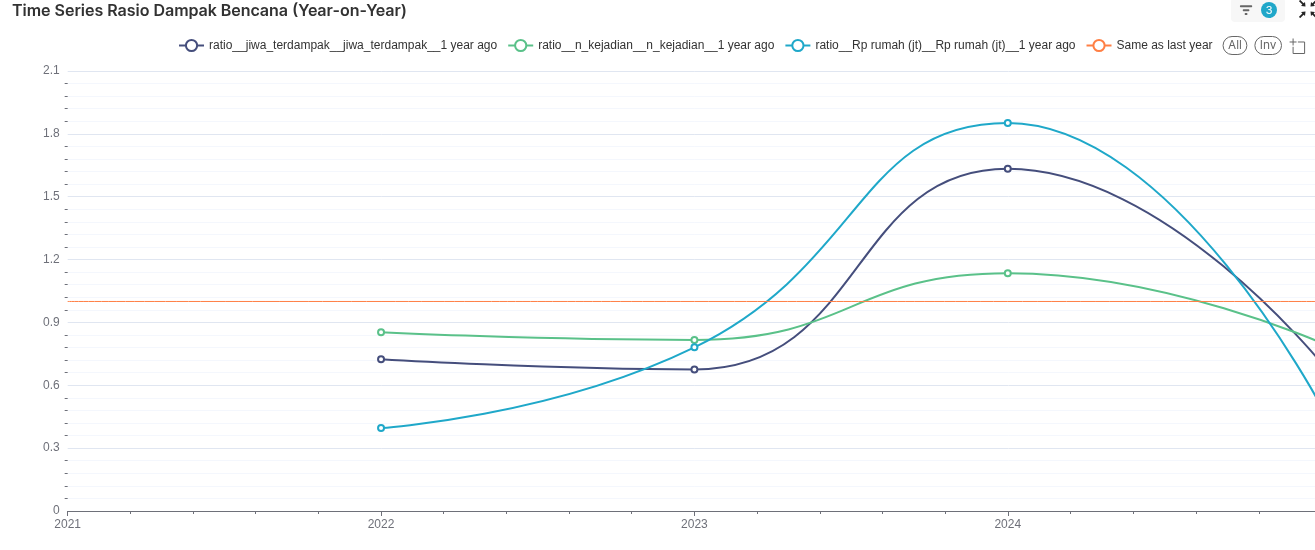
\includegraphics[width=0.8\linewidth]{fig3.png}}
    \caption{Impact caused by floods in Indonesia (mio IDR)}
    \label{fig:floodimpact}
    \vspace{0.2cm}
\footnotesize{\textit{Source:} \url{https://dibi.bnpb.go.id}}
\end{figure}

Moreover, research on risk management within emergency supply chains remains scarce. Many existing studies lack the practical and integrated methodologies needed to support real-time decision-making under conditions of uncertainty \cite{chukwuka2023comprehensive}. This gap underscores the necessity for intelligent decision support tools capable of managing disruptions in complex humanitarian logistics environments.

One such emerging approach is the development of resilient supply chains, defined as systems that can recover and return to normal operations within an acceptable timeframe following a disruption \cite{orengo2022food}. Building this resilience requires not only robust planning but also adaptive, intelligent frameworks that can prioritize needs dynamically and optimize resource allocation in real time.

This study addresses these challenges by proposing a simulation-based Decision Support System (DSS) that integrates fuzzy inference and a greedy algorithm to provide a rapid, adaptive response mechanism during natural disasters. The system is designed to improve the responsiveness and efficiency of humanitarian supply chains through real-time prioritization and resource allocation. To support this, the simulation utilizes data from the Indonesian National Statistics Agency (BPS) and historical disaster records from the National Disaster Management Authority (BNPB) to identify high-risk regions and evaluate logistical response scenarios.

\section{Literature Review}

Decision Support Systems (DSS) have become increasingly important in disaster management, providing tools for effective decision-making under uncertainty \cite{khan2023systematic}. These systems integrate data analysis, modeling, and simulation to support emergency response\cite{alghodhaifi2021autonomous}. The use of DSS in disaster management has been shown to enhance situational awareness, improve coordination among stakeholders, and optimize logistics operations \cite{adetiloye2021collaboration}. For instance, Peron et al. (2022) demonstrated the effectiveness of a DSS in workforce management \cite{peron2022decision}. During disaster response, highlighting the importance of integrating demographic data and historical disaster records to inform decision-making\cite{suarez2024integrated}.

Simulation-based approaches are widely used in disaster management to evaluate the performance of DSS and assess various scenarios without the need for real-world implementation \cite{chang2022simulation}. These approaches allow for the modeling of complex systems and the assessment of different disaster scenarios, enabling decision-makers to identify the most affected regions and the number of victims. For example, Lobkov et al. (2023) utilized simulation techniques to estimate the impact of disasters on affected populations, demonstrating the importance of accurate data collection and processing in disaster response planning \cite{lobkov2023determination}. 

Fuzzy Inference Systems (FIS) are employed to assess the severity and urgency of disasters, providing a flexible framework for decision-making under uncertainty \cite{anjomshoae2021integrated}. 
Understanding fuzzy logic is crucial for developing effective DSS, as it allows for the incorporation of expert knowledge and subjective assessments, enabling the system to handle imprecise and ambiguous data effectively\cite{improta2020fuzzy}. 

Crisp input values are converted into fuzzy values using membership functions. A trapezoidal membership function is defined as:

\[
\mu_A(x) = 
\begin{cases}
0, & x \leq a \\
\frac{x - a}{b - a}, & a < x < b \\
1, & b \leq x \leq c \\
\frac{d - x}{d - c}, & c < x < d \\
0, & x \geq d
\end{cases}
\]

The fuzzy inference uses logical operators such as \textit{AND} and \textit{OR}. For example, for the \textbf{AND} operator (min function):

\[
\mu_{\text{Rule}} = \min\left( \mu_{\text{Health}}(x), \mu_{\text{Age}}(y), \mu_{\text{Risk}}(z) \right)
\]

If multiple rules produce output sets, they are combined using the max operator:

\[
\mu_{\text{Output}}(z) = \max \left( \mu_{\text{Rule}_1}(z), \mu_{\text{Rule}_2}(z),.., \mu_{\text{Rule}_n}(z) \right)
\]

To obtain a crisp output, the Centroid (Center of Gravity) method is commonly used:

\[
z^* = \frac{\int z \cdot \mu(z) \, dz}{\int \mu(z) \, dz}
\]

Where:
\begin{itemize}
    \item \( z^* \) is the defuzzified output (e.g., prioritization score),
    \item \( \mu(z) \) is the aggregated membership function of the output.
\end{itemize}

Fuzzy logic allows for the incorporation of expert knowledge and subjective assessments, enabling the system to handle imprecise and ambiguous data effectively \cite{jain2020membership}. The use of fuzzy rules to determine the relationship between independent and dependent variables has been shown to enhance the accuracy of disaster impact assessments \cite{yoon2023novel}.


\section{Methodology}
\subsection{Data Simulation}

Many studies involves a simulation-based approach to evaluate the performance of a Decision Support System (DSS)\cite{he2020dynamic}. This approach allows for the modeling of complex systems and the assessment of various scenarios without the need for real-world implementation\cite{latchmore2023integrating}. This study collects and processes data from the Indonesian National Statistics Agency (BPS) and the National Disaster Management Authority (BNPB) to simulate disaster scenarios. Determining the most affected regions and the number of victims is crucial for effective disaster response planning \cite{endo2020estimating}. The simulation framework incorporates demographic data, historical disaster records, and geographical information \cite{santos2020workforce}. Determining the most affected regions and the number of victims is shown in Figure~\ref{fig:simulationframework}. 
\begin{figure}[htbp]
    \centerline{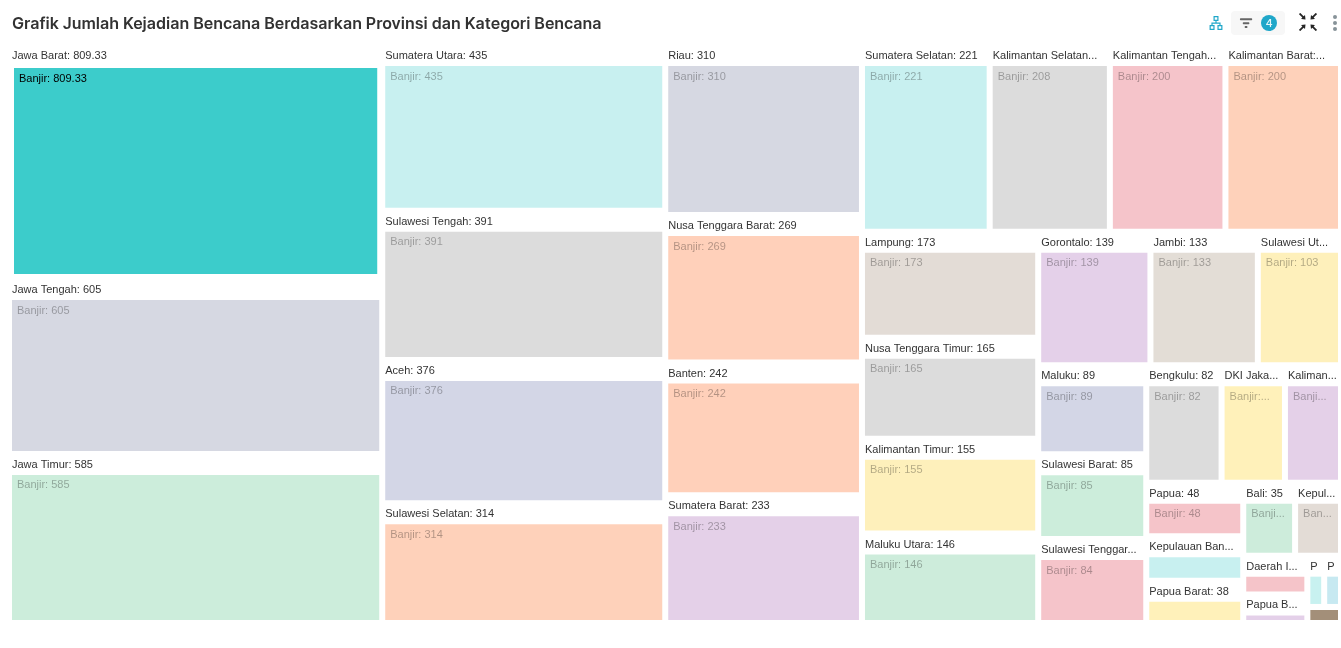
\includegraphics[width=0.8\linewidth]{fig4.png}
    }
    \caption{Most Affected Regions in 2021 - 2025}
    \label{fig:simulationframework}
    \footnotesize{\textit{Source:} \url{https://dibi.bnpb.go.id}}
\end{figure}

Based on heatmap the west Java region is the most occurrences based on floods natural disaster, then districs of Bogor, Bandung, and Bekasi are the most affected areas, can be shwon in Figure~\ref{fig:heatmap2}. 
\begin{figure}[htbp]
    \centerline{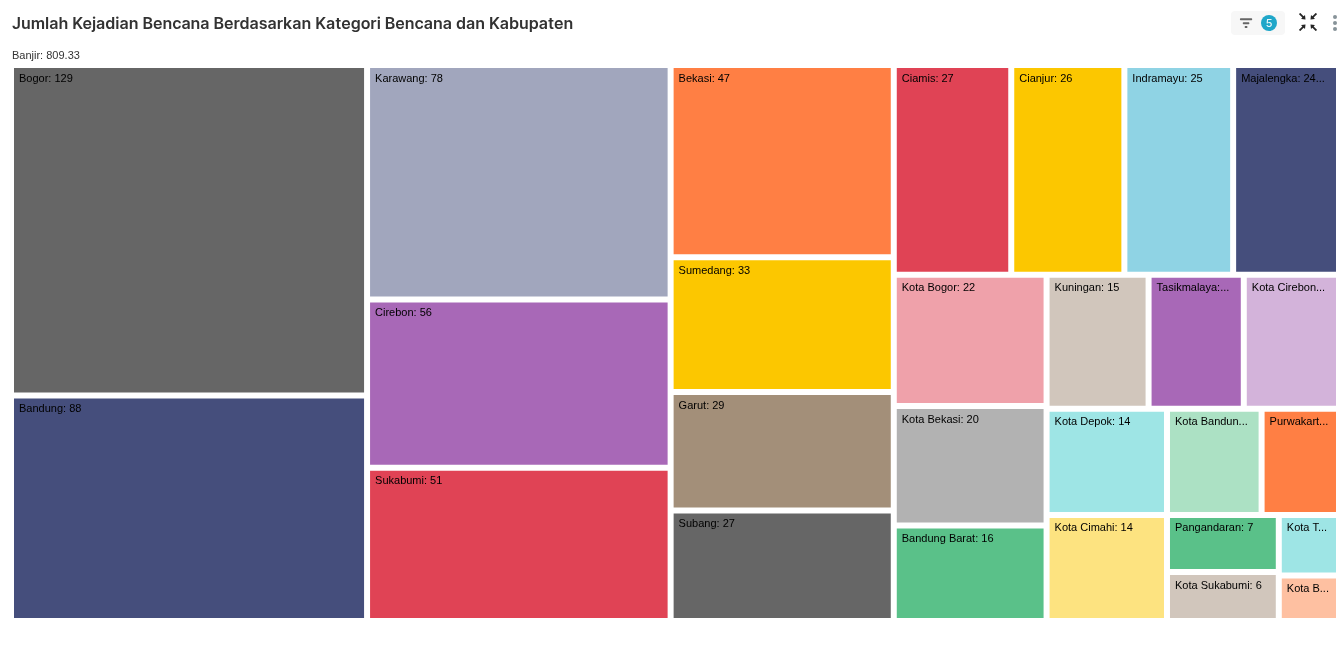
\includegraphics[width=0.8\linewidth]{fig5.png}}
    \caption{Heatmap of Floods in West Java in 2021 - 2025}
    \label{fig:heatmap2}
    \footnotesize{\textit{Source:} \url{https://dibi.bnpb.go.id}}
\end{figure} 

Making sure that the simulation accurately reflects the real-world conditions faced during disaster response operations. Spatial analysis hydrological data is also integrated to assess the impact of floods \cite{alkaesi2021spatial}. Result of analysis is shown in table \ref{tab:analysis}.
\begin{table}[htbp]
\caption{Runoff Flooding Potential by Sub-district in Bogor Region}
\begin{center}
\begin{tabular}{|m{2.5cm}|m{2cm}|}
\hline
\textbf{Sub-district} & \textbf{Flood Potential} \\
\hline
Nanggung & Extreme \\
\hline Sukajaya & Extreme  \\
\hline Sukamakmur & Extreme \\
\hline Tanjungsari & Extreme \\
\hline Cigudeg & Extreme  \\
\hline Megamendung & Extreme  \\
\hline Babakanmadang & Extreme  \\
\hline
Cigudeg & High \\
\hline Pamijahan & High  \\
\hline Sukajaya & High  \\
\hline Sukamakmur & High\\
\hline
Jasinga & Low/Normal  \\
\hline Rumpin & Low/Normal  \\
\hline Tejo Panjang & Low/Normal  \\
\hline
\end{tabular}
\vspace{0.2cm}

\footnotesize{\textit{Source:} Adapted from \cite{alkaesi2021spatial}.}
\label{tab:analysis}
\end{center}
\end{table}

Based on the analysis, the simulation will be taken on sub districs are identified as having extreme ,high, and normal flood potential. This information is used in simulation after adding demographic data from BPS, which includes population density and socio-economic indicators. The simulation framework is designed to model the logistics and supply chain operations during disaster response, focusing on the allocation of resources and routing of aid based on the severity and urgency of the situation \cite{park2021architectural}. Warehouse locations is based on the proximity to affected areas, ensuring that resources can be deployed quickly and efficiently \cite{halawa2020introduction}.  

\subsection{Fuzzy Inference System (FIS) and Greedy Algorithm}
The Fuzzy Inference System (FIS) is employed to assess the severity and urgency of disasters, providing a flexible framework for decision-making under uncertainty \cite{berawi2020prioritized}. According Berawi et al. following Fuzzy rules are generated :

\begin{itemize}
    \item IF Healthy Level is \textbf{Sick}, AND Age is \textbf{Adult} or \textbf{Kid}, AND Risk Level is \textbf{High} or \textbf{Moderate}, THEN the victim is \textbf{Prioritized}.
    
    \item IF Healthy Level is \textbf{Sick}, AND Age is \textbf{Adult} or \textbf{Kid}, AND Risk Level is \textbf{Low}, THEN the victim is \textbf{Prioritized}.
    
    \item IF Healthy Level is \textbf{Sick}, AND Age is \textbf{Elder}, AND Distance is \textbf{Far} or \textbf{Nearby}, THEN the victim is \textbf{Prioritized}.
    
    \item IF Healthy Level is \textbf{Sick}, AND Age is \textbf{Elder}, AND Distance is \textbf{Moderate}, THEN the victim is \textbf{Prioritized}.
    
    \item IF Healthy Level is \textbf{Healthy} or \textbf{Okay}, AND Age is \textbf{Elder} or \textbf{Kid}, AND Risk Level is \textbf{Moderate}, THEN the victim is \textbf{not Prioritized}.
    
    \item IF Healthy Level is \textbf{Healthy} or \textbf{Okay}, AND Age is \textbf{Elder} or \textbf{Kid}, AND Risk Level is \textbf{High}, THEN the victim is \textbf{not Prioritized}.
    
    \item IF Healthy Level is \textbf{Healthy} or \textbf{Okay}, AND Age is \textbf{Adult}, THEN the victim is \textbf{not Prioritized}.
\end{itemize}


Fuzzy logic allows for the incorporation of expert knowledge and subjective assessments, enabling the system to handle imprecise and ambiguous data effectively \cite{jain2020membership}. The model is highly flexible and can be adjusted according to the actual conditions of the damaged area. In the development of the membership function, contextual parameters must be carefully defined based on observed field data \cite{amiri2021application}. fuzzy rules were made to determine the relationship between independent and dependent variables \cite{yoon2023novel}. The rules are defined based on expert knowledge and historical data, allowing the system to evaluate the impact of disasters on affected regions \cite{wang2024gis}. This study use SPHERE handbook as a reference for the fuzzy rules, which are designed to prioritize disaster impact zones based on severity, urgency, and accessibility \cite{sphere2018pdf}. Table \ref{tab:dependent_variables_sphere} is dependent variables from SPHERE handbook.

\begin{table}[H]
\caption{Potential Dependent Variables Aligned with the Sphere Handbook Principles}
\begin{center}
\begin{tabular}{|p{2cm}|p{2cm}|p{2cm}|}
\hline
\textbf{Dependent Variable} & \textbf{Description} & \textbf{Relevance to Sphere Handbook} \\
\hline
Response Time & Time required to deliver aid to affected populations (e.g., hours) & Timeliness and accessibility of humanitarian assistance \\
\hline
Coverage of Affected Population & Proportion (\%) of disaster victims who receive aid & Non-discrimination, equity, and universal access \\
\hline
Logistics Efficiency & Efficiency in terms of cost, distance, or load (e.g., ton/km or cost per beneficiary) & Effective resource utilization and accountability \\
\hline
Unmet Needs Score & Index measuring the gap in critical needs (e.g., shelter, food, WASH) & Fulfillment of minimum humanitarian standards \\
\hline
Protection or Satisfaction Index & Victim-reported perception of safety, dignity, and fairness (via surveys or scoring) & Protection, dignity, and community engagement \\
\hline
\end{tabular}
\label{tab:dependent_variables_sphere}
\end{center}
\end{table}


After rules are defined, the FIS is implemented using the Mamdani method, which is suitable for handling complex and non-linear relationships in disaster scenarios \cite{herpratiwi2022implementation}. Greedy algorithm is used to optimize resource allocation and routing based on the priority indices generated by the FIS \cite{shirmarz2020adaptive}. The greedy algorithm is chosen for its efficiency in finding near-optimal solutions in complex logistics problems, particularly in dynamic environments where rapid decision-making is crucial \cite{hamidouglu2023game}. The combination of FIS and greedy algorithm allows for a robust decision support system that can adapt to changing conditions and prioritize resources effectively during disaster response operations. 
 

\subsection{Research Framework}

This study adopts a simulation-based quantitative approach to evaluate the performance of an intelligent decision support system (DSS) in the context of humanitarian logistics for disaster response. The framework consists of three major components: data driven acquisition, DSS algorithms, and simulation-based evaluation \cite{mahmoodi2024data}. Figure \ref{fig:research_framework} illustrates the research framework, which integrates data acquisition, fuzzy inference, greedy algorithm, and simulation to assess the effectiveness of the proposed DSS in disaster response scenarios.

\begin{figure}[htbp]
\centering
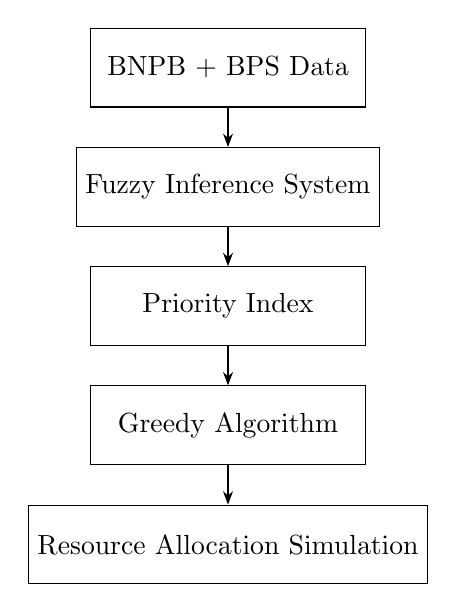
\begin{tikzpicture}[
    node distance=0.5cm and 1cm,
    box/.style={rectangle, draw, minimum width=3.5cm, minimum height=1cm, align=center},
    ->, >=Stealth
  ]

% Nodes
\node[box] (data) {BNPB + BPS Data};
\node[box, below=of data] (fuzzy) {Fuzzy Inference System};
\node[box, below=of fuzzy] (priority) {Priority Index};
\node[box, below=of priority] (greedy) {Greedy Algorithm};
\node[box, below=of greedy] (sim) {Resource Allocation Simulation};

% Arrows
\draw[->] (data) -- (fuzzy);
\draw[->] (fuzzy) -- (priority);
\draw[->] (priority) -- (greedy);
\draw[->] (greedy) -- (sim);

\end{tikzpicture}
\caption{Research Framework Flow: From Data to Simulation Output}
\label{fig:research_framework}
\end{figure}

The system receives input data from two key sources: the Indonesian National Statistics Agency (BPS), which provides demographic and regional data, and the National Disaster Management Authority (BNPB), which offers historical records of disaster occurrences. This data is processed and transformed into relevant indicators such as disaster severity, urgency, accessibility, and population density.

These indicators serve as inputs to a Fuzzy Inference System (FIS), which generates a priority index for each affected region. The FIS captures the uncertainty and complexity inherent in disaster impact assessment through a rule-based system of fuzzy logic. The resulting priority scores are then passed to a greedy algorithm that rapidly determines the optimal routing or allocation of resources based on proximity and urgency.

The entire process is simulated using various disaster scenarios to assess system performance in terms of response time, supply coverage, and the number of affected individuals reached. This research framework allows for comprehensive evaluation of the hybrid DSS under dynamic, high-stakes conditions, providing insights into its practical applicability for emergency logistics operations.

\section{Results and Discussion}

\section{Conclusion}


\section*{Acknowledgment}

The preferred spelling of the word ``acknowledgment'' in America is without 
an ``e'' after the ``g''. Avoid the stilted expression ``one of us (R. B. 
G.) thanks $\ldots$''. Instead, try ``R. B. G. thanks$\ldots$''. Put sponsor 
acknowledgments in the unnumbered footnote on the first page.



\bibliographystyle{IEEEtran}
\bibliography{references} 
%(note: if you want to add the references, please do not forget to change the name of the reference in \bibliography{Name_References} according to author's name of reference file. For example, if the name is John_References, it becomes \bibliography{John_References})




\label{lastPage}

\end{document}
